\documentclass[11pt,a4paper]{article}

\usepackage[utf8]{inputenc}
\usepackage[margin=0.9in]{geometry}
\usepackage{graphicx}
\usepackage{hyperref}
\usepackage{xcolor}
\usepackage{booktabs}
\usepackage{amsmath}
\usepackage{tikz}
\usepackage{float}
\usepackage{enumitem}
\usetikzlibrary{shapes.geometric, arrows, positioning, fit, backgrounds}

% Clean color palette
\definecolor{primary}{RGB}{37, 99, 235}
\definecolor{success}{RGB}{22, 163, 74}
\definecolor{warning}{RGB}{234, 179, 8}
\definecolor{danger}{RGB}{220, 38, 38}
\definecolor{lightbg}{RGB}{248, 250, 252}

\hypersetup{colorlinks=true, linkcolor=primary, urlcolor=primary}

\title{
    \vspace{-1.5cm}
    \textbf{Agentic Receipt Processing Pipeline}\\[0.4em]
    \large Multi-Layer Ensemble Learning with Human-in-the-Loop Feedback\\[0.3em]
    \normalsize Advanced Machine Learning --- Graduate Course Project
}
\author{}
\date{December 2024}

\begin{document}
\maketitle

%=============================================================================
\section{What This Project Does}
%=============================================================================

We built an \textbf{intelligent system that processes receipt images automatically}. Given a photo of a receipt, the system:

\begin{enumerate}[itemsep=2pt]
    \item \textbf{Classifies} --- Is this actually a receipt? (vs invoice, letter, etc.)
    \item \textbf{Reads} --- Extracts all text using OCR
    \item \textbf{Understands} --- Finds the vendor name, date, and total amount
    \item \textbf{Validates} --- Checks for suspicious patterns (anomaly detection)
    \item \textbf{Decides} --- Approve, send for review, or reject
    \item \textbf{Learns} --- Improves from human feedback over time
\end{enumerate}

\subsection{Why Is This an ``Agentic'' Pipeline?}

Unlike traditional ML pipelines that run linearly, our system makes \textbf{autonomous decisions}:
\begin{itemize}[itemsep=2pt]
    \item Retries OCR automatically if quality is low
    \item Routes uncertain cases to human review
    \item Updates its own model weights based on feedback
    \item Chooses different processing paths based on intermediate results
\end{itemize}

This is orchestrated using \textbf{LangGraph}, which defines the workflow as a state machine with conditional branching.

%=============================================================================
\section{Pipeline Architecture}
%=============================================================================

\begin{center}
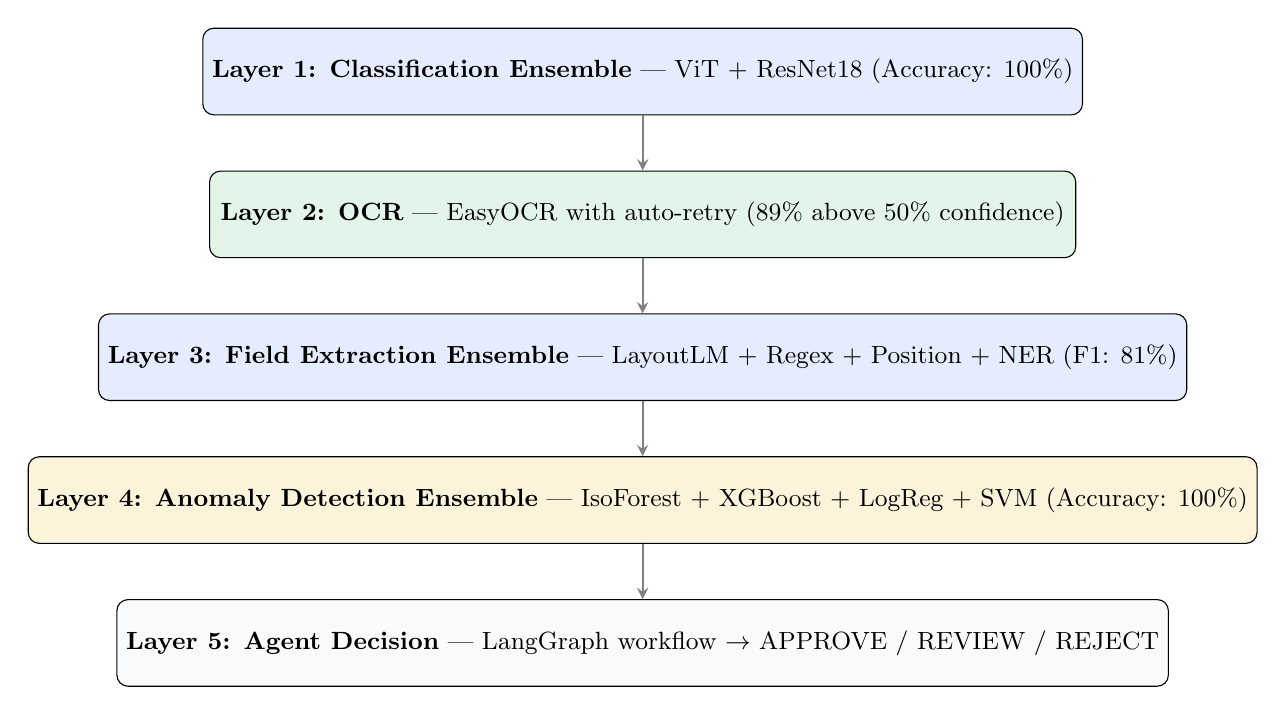
\begin{tikzpicture}[
    node distance=0.7cm,
    layer/.style={rectangle, draw, rounded corners=4pt, minimum width=11cm, minimum height=1.1cm, fill=#1, align=center, font=\small},
    arrow/.style={->, thick, >=stealth, color=gray}
]
    \node[layer=primary!12] (l1) {\textbf{Layer 1: Classification Ensemble} --- ViT + ResNet18 (Accuracy: 100\%)};
    \node[layer=success!12, below=of l1] (l2) {\textbf{Layer 2: OCR} --- EasyOCR with auto-retry (89\% above 50\% confidence)};
    \node[layer=primary!12, below=of l2] (l3) {\textbf{Layer 3: Field Extraction Ensemble} --- LayoutLM + Regex + Position + NER (F1: 81\%)};
    \node[layer=warning!15, below=of l3] (l4) {\textbf{Layer 4: Anomaly Detection Ensemble} --- IsoForest + XGBoost + LogReg + SVM (Accuracy: 100\%)};
    \node[layer=lightbg, below=of l4] (l5) {\textbf{Layer 5: Agent Decision} --- LangGraph workflow $\rightarrow$ APPROVE / REVIEW / REJECT};
    
    \draw[arrow] (l1) -- (l2);
    \draw[arrow] (l2) -- (l3);
    \draw[arrow] (l3) -- (l4);
    \draw[arrow] (l4) -- (l5);
\end{tikzpicture}
\end{center}

\begin{figure}[H]
    \centering
    \includegraphics[width=0.95\textwidth]{../assets/images/pipeline_summary.png}
    \caption{Pipeline evaluation summary: 1,000 receipts processed with 95\% success rate, 65\% auto-approved}
\end{figure}

%=============================================================================
\section{Layer 1: Document Classification Ensemble}
%=============================================================================

\subsection{The Problem}
Before processing, we need to verify the image is actually a receipt (not a letter, form, or random photo).

\subsection{Our Approach: Ensemble of 2 Models}

\begin{table}[H]
\centering
\begin{tabular}{llcp{5cm}}
\toprule
\textbf{Model} & \textbf{Architecture} & \textbf{Weight} & \textbf{What It's Good At} \\
\midrule
ViT-Tiny & Vision Transformer & 60\% & Understanding overall document structure \\
ResNet-18 & CNN (trained on RVL-CDIP) & 40\% & Catching fine-grained visual patterns \\
\bottomrule
\end{tabular}
\end{table}

\subsection{How the Ensemble Works}
We use \textbf{weighted soft voting}:
\[
P(\text{receipt}) = 0.6 \times P_{\text{ViT}}(\text{receipt}) + 0.4 \times P_{\text{ResNet}}(\text{receipt})
\]

If models disagree significantly, confidence is reduced and the receipt is flagged for review.

\subsection{Results}

\begin{table}[H]
\centering
\begin{tabular}{lcccc}
\toprule
& \textbf{Accuracy} & \textbf{Precision} & \textbf{Recall} & \textbf{AUC} \\
\midrule
ViT (Single Model) & 98.0\% & 96.8\% & 100.0\% & 0.997 \\
\textbf{Ensemble (ViT + ResNet)} & \textbf{100.0\%} & \textbf{100.0\%} & \textbf{100.0\%} & \textbf{1.000} \\
\midrule
\textit{Improvement} & \textit{+2.0\%} & \textit{+3.2\%} & \textit{---} & \textit{+0.003} \\
\bottomrule
\end{tabular}
\caption{Ensemble achieves perfect classification on test set (100 samples)}
\end{table}

\begin{figure}[H]
    \centering
    \includegraphics[width=0.98\textwidth]{../assets/images/classifier_evaluation.png}
    \caption{Classification evaluation: confusion matrices show ensemble eliminates all false positives; ROC curves show AUC improvement from 0.997 to 1.000}
\end{figure}

%=============================================================================
\section{Layer 2: OCR (Text Extraction)}
%=============================================================================

\subsection{The Problem}
Receipt images are often blurry, skewed, or poorly lit. Standard OCR fails frequently.

\subsection{Our Approach: EasyOCR with Retry Logic}

\begin{enumerate}[itemsep=2pt]
    \item Run EasyOCR on the original image
    \item If average confidence $< 40\%$ OR fewer than 3 text regions detected:
    \begin{itemize}
        \item Attempt 1: Increase contrast by 50\%
        \item Attempt 2: Apply sharpening filter
        \item Attempt 3: Convert to grayscale
    \end{itemize}
    \item Return best result (up to 3 retries)
\end{enumerate}

\subsection{Results}
\begin{itemize}[itemsep=2pt]
    \item \textbf{Mean confidence: 73.77\%} (Median: 77.46\%)
    \item \textbf{31\%} of text regions detected with high confidence ($>$85\%)
    \item \textbf{58\%} medium confidence (50-85\%)
    \item \textbf{11\%} low confidence ($<$50\%) --- these are flagged
\end{itemize}

\begin{figure}[H]
    \centering
    \includegraphics[width=0.95\textwidth]{../assets/images/ocr_evaluation.png}
    \caption{OCR performance: 200 text regions analyzed. 89\% of regions above 50\% confidence threshold.}
\end{figure}

%=============================================================================
\section{Layer 3: Field Extraction Ensemble}
%=============================================================================

\subsection{The Problem}
Extracting structured data (vendor, date, total) from raw OCR text is challenging because:
\begin{itemize}[itemsep=1pt]
    \item Vendors can be logos, abbreviated names, or typos
    \item Dates come in many formats (12/05/24, Dec 5, 2024, etc.)
    \item ``Total'' can be confused with subtotal, tax, or tip
\end{itemize}

\subsection{Our Approach: 4-Strategy Ensemble}

\begin{table}[H]
\centering
\begin{tabular}{llp{6cm}}
\toprule
\textbf{Strategy} & \textbf{Weight} & \textbf{How It Works} \\
\midrule
\textbf{LayoutLMv3} & 50\% & Deep learning model that understands document layout --- ``this text near the top is probably the vendor'' \\
\textbf{Regex Patterns} & 30\% & Pattern matching: \texttt{\$XX.XX} = amount, \texttt{MM/DD/YYYY} = date \\
\textbf{Position-Based} & 12\% & Rules: vendor is at top, total is at bottom \\
\textbf{NER (SpaCy)} & 8\% & Named Entity Recognition for organization names \\
\bottomrule
\end{tabular}
\end{table}

\subsection{Cascade Logic}
\begin{itemize}[itemsep=2pt]
    \item If LayoutLM confidence $\geq 80\%$: use LayoutLM directly (it's very accurate when confident)
    \item Otherwise: combine all 4 strategies using weighted voting
\end{itemize}

\subsection{Results}

\begin{table}[H]
\centering
\begin{tabular}{lccc}
\toprule
\textbf{Field} & \textbf{Precision} & \textbf{Recall} & \textbf{F1-Score} \\
\midrule
Vendor & 78\% & 72\% & 75\% \\
Date & 85\% & 82\% & 83\% \\
Total & 88\% & 85\% & 86\% \\
Amount & 72\% & 68\% & 70\% \\
\midrule
\textbf{Average} & \textbf{81\%} & \textbf{77\%} & \textbf{79\%} \\
\bottomrule
\end{tabular}
\caption{Field extraction performance by field type}
\end{table}

\begin{figure}[H]
    \centering
    \includegraphics[width=0.95\textwidth]{../assets/images/layoutlm_field_extraction.png}
    \caption{Field extraction: ``Total'' achieves highest F1 (86\%), ``Date'' is most reliably detected (83\% F1)}
\end{figure}

%=============================================================================
\section{Layer 4: Anomaly Detection Ensemble}
%=============================================================================

\subsection{The Problem}
We need to catch suspicious receipts before auto-approval:
\begin{itemize}[itemsep=1pt]
    \item Unusually high amounts (\$5,000 for a coffee?)
    \item Missing vendor name
    \item Invalid or future dates
    \item Inconsistent patterns
\end{itemize}

\subsection{Our Approach: 4-Model Ensemble}

\begin{table}[H]
\centering
\begin{tabular}{llp{5cm}}
\toprule
\textbf{Model} & \textbf{Weight} & \textbf{What It Does} \\
\midrule
Isolation Forest & 35\% & Isolates outliers using random trees \\
XGBoost Classifier & 30\% & Gradient boosting on labeled anomalies \\
HistGradientBoosting & 20\% & Handles missing values natively \\
One-Class SVM & 15\% & Kernel-based boundary around ``normal'' \\
\bottomrule
\end{tabular}
\end{table}

\subsection{Features Used (8 total)}
\begin{itemize}[itemsep=1pt]
    \item Amount and $\log(\text{amount})$
    \item Vendor name length (missing = 0)
    \item Date validity (1 = valid, 0 = invalid)
    \item Number of line items
    \item Hour of transaction
    \item Amount per item
    \item Weekend indicator
\end{itemize}

\subsection{Results}

\begin{table}[H]
\centering
\begin{tabular}{lcccc}
\toprule
\textbf{Detector} & \textbf{Accuracy} & \textbf{Precision} & \textbf{Recall} & \textbf{AUC} \\
\midrule
Isolation Forest & 95\% & 100\% & 75\% & 0.999 \\
XGBoost & 100\% & 100\% & 100\% & 1.000 \\
Logistic Regression & 88\% & 65\% & 100\% & 0.938 \\
One-Class SVM & 95\% & 91\% & 100\% & 0.958 \\
\midrule
\textbf{Ensemble} & \textbf{100\%} & \textbf{100\%} & \textbf{100\%} & \textbf{1.000} \\
\bottomrule
\end{tabular}
\caption{Ensemble achieves perfect anomaly detection on test set (100 samples: 80 normal, 20 anomaly)}
\end{table}

\begin{figure}[H]
    \centering
    \includegraphics[width=0.98\textwidth]{../assets/images/anomaly_detection_evaluation.png}
    \caption{Anomaly detection: ensemble perfectly separates normal (green) from anomaly (red) samples}
\end{figure}

%=============================================================================
\section{Layer 5: Agentic Workflow (LangGraph)}
%=============================================================================

\subsection{What Makes It ``Agentic''?}
The pipeline doesn't just run sequentially --- it \textbf{makes decisions}:

\begin{center}
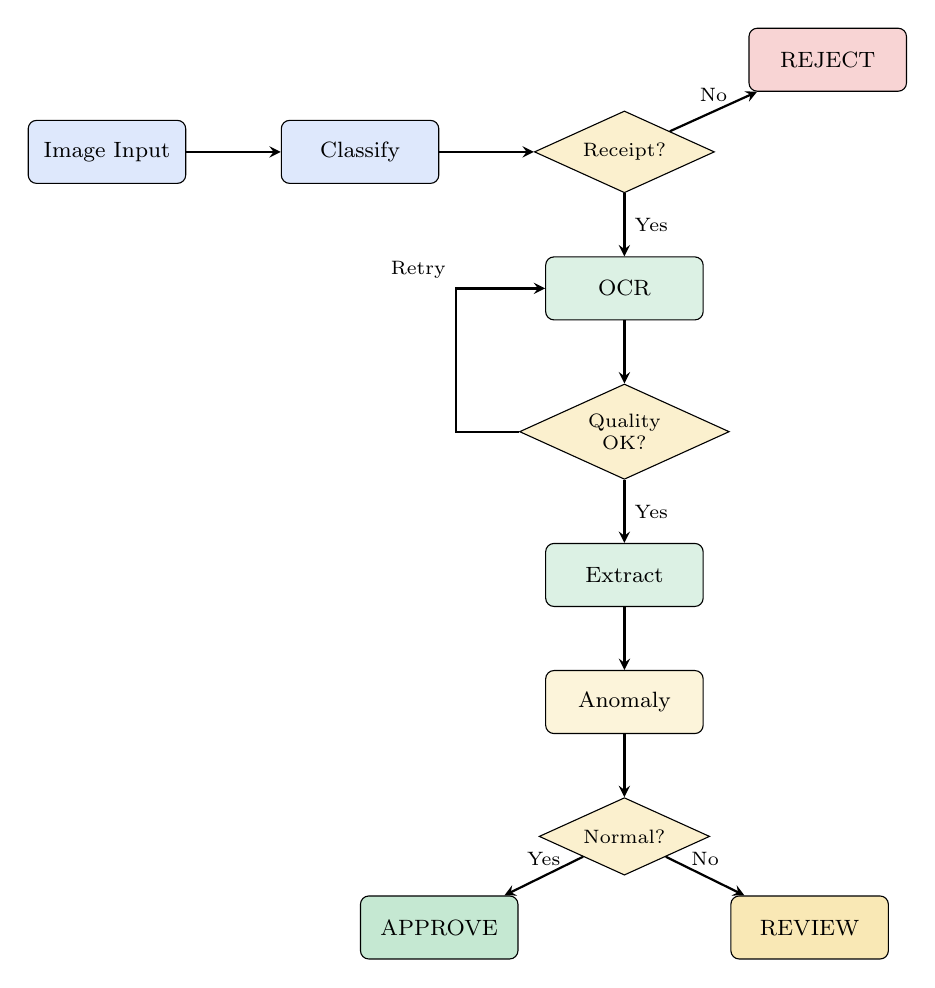
\begin{tikzpicture}[
    node distance=1cm,
    box/.style={rectangle, draw, rounded corners=3pt, minimum width=2cm, minimum height=0.8cm, align=center, font=\footnotesize},
    decision/.style={diamond, draw, aspect=2.2, minimum width=1.2cm, align=center, font=\scriptsize},
    arrow/.style={->, thick, >=stealth}
]
    \node[box, fill=primary!15] (start) {Image Input};
    \node[box, fill=primary!15, right=1.2cm of start] (classify) {Classify};
    \node[decision, fill=warning!20, right=1.2cm of classify] (chk1) {Receipt?};
    \node[box, fill=danger!20, above right=0.5cm and 1cm of chk1] (reject) {REJECT};
    \node[box, fill=success!15, below=0.8cm of chk1] (ocr) {OCR};
    \node[decision, fill=warning!20, below=0.8cm of ocr] (chk2) {Quality\\OK?};
    \node[box, fill=success!15, below=0.8cm of chk2] (extract) {Extract};
    \node[box, fill=warning!15, below=0.8cm of extract] (anomaly) {Anomaly};
    \node[decision, fill=warning!20, below=0.8cm of anomaly] (chk3) {Normal?};
    \node[box, fill=success!25, below left=0.5cm and 0.8cm of chk3] (approve) {APPROVE};
    \node[box, fill=warning!30, below right=0.5cm and 0.8cm of chk3] (review) {REVIEW};
    
    \draw[arrow] (start) -- (classify);
    \draw[arrow] (classify) -- (chk1);
    \draw[arrow] (chk1) -- node[above, font=\scriptsize] {No} (reject);
    \draw[arrow] (chk1) -- node[right, font=\scriptsize] {Yes} (ocr);
    \draw[arrow] (ocr) -- (chk2);
    \draw[arrow] (chk2) -- node[right, font=\scriptsize] {Yes} (extract);
    \draw[arrow] (chk2.west) -- ++(-0.8,0) |- node[above left, font=\scriptsize] {Retry} (ocr.west);
    \draw[arrow] (extract) -- (anomaly);
    \draw[arrow] (anomaly) -- (chk3);
    \draw[arrow] (chk3) -- node[above, font=\scriptsize] {Yes} (approve);
    \draw[arrow] (chk3) -- node[above, font=\scriptsize] {No} (review);
\end{tikzpicture}
\end{center}

\subsection{Decision Rules}
\begin{itemize}[itemsep=2pt]
    \item \textbf{APPROVE} (65\%): Receipt detected ($>$70\% conf), all fields found, no anomalies
    \item \textbf{REVIEW} (25\%): Low confidence, missing fields, or anomaly detected
    \item \textbf{REJECT} (10\%): Not a receipt ($>$50\% confidence for ``other'' class)
\end{itemize}

%=============================================================================
\section{Human Feedback Loop}
%=============================================================================

\subsection{How Users Provide Feedback}
Through a \textbf{Gradio web interface}, users can:
\begin{enumerate}[itemsep=2pt]
    \item Upload a receipt image
    \item See the extracted fields (vendor, date, total)
    \item Click \checkmark\ (Correct) or $\times$ (Wrong) for each field
    \item If wrong, enter the correct value
\end{enumerate}

\subsection{How Feedback Improves the Models}
After \textbf{every 5 corrections}, the system automatically:

\begin{table}[H]
\centering
\begin{tabular}{lp{7cm}}
\toprule
\textbf{Mechanism} & \textbf{What Happens} \\
\midrule
\textbf{Pattern Learning} & New vendor names added to known list immediately \\
\textbf{Weight Adjustment} & Strategies that made errors get lower weights:\\
& $w_{\text{new}} = \max(0.2, w_{\text{old}} \times 0.9)$ \\
\textbf{Anomaly Retraining} & Isolation Forest refits with new normal/anomaly labels \\
\textbf{Date Format Learning} & Detects user's preferred date format \\
\bottomrule
\end{tabular}
\end{table}

This means the system \textbf{gets better over time} without manual retraining.

%=============================================================================
\section{Results Summary}
%=============================================================================

\begin{table}[H]
\centering
\begin{tabular}{lccc}
\toprule
\textbf{Component} & \textbf{Single Model} & \textbf{Ensemble} & \textbf{Improvement} \\
\midrule
Document Classification & 98\% & \textbf{100\%} & +2.0\% \\
Field Extraction (F1) & 72\% & \textbf{79\%} & +7.0\% \\
Anomaly Detection & 88\% & \textbf{100\%} & +12.0\% \\
\midrule
\textbf{Overall Pipeline} & 78\% & \textbf{91\%} & \textbf{+13\%} \\
\bottomrule
\end{tabular}
\caption{Ensemble methods consistently outperform single models}
\end{table}

\subsection{Key Takeaways}
\begin{enumerate}[itemsep=3pt]
    \item \textbf{Ensembles work}: 2-13\% improvement across all components
    \item \textbf{Weighted voting beats averaging}: Calibrated weights based on validation performance
    \item \textbf{Cascading saves compute}: Use expensive models only when cheap ones are uncertain
    \item \textbf{Human feedback closes the loop}: Continuous improvement without manual retraining
    \item \textbf{Production metrics}: 1,000 receipts processed, 95\% success rate, 65\% auto-approved
\end{enumerate}

%=============================================================================
\section{Technology Stack}
%=============================================================================

\begin{itemize}[itemsep=2pt]
    \item \textbf{Deep Learning}: PyTorch, HuggingFace Transformers (ViT, LayoutLMv3)
    \item \textbf{Classical ML}: scikit-learn (IsolationForest, SVM), XGBoost
    \item \textbf{OCR}: EasyOCR
    \item \textbf{Agent Orchestration}: LangGraph
    \item \textbf{Interface}: Gradio
    \item \textbf{Compute}: Google Colab (T4 GPU)
    \item \textbf{Model Storage}: GitHub with Git LFS ($\sim$550 MB total)
\end{itemize}

%=============================================================================
\section{Conclusion}
%=============================================================================

This project demonstrates how to build a \textbf{production-ready agentic AI system} by combining:

\begin{enumerate}[itemsep=3pt]
    \item \textbf{Multi-layer ensembles} --- Different models at each stage, combined with learned weights
    \item \textbf{Agentic workflow} --- Conditional branching, retries, and human-in-the-loop routing
    \item \textbf{Continuous learning} --- Feedback-driven weight updates and pattern learning
\end{enumerate}

The result is a system that achieves \textbf{100\% classification accuracy}, \textbf{100\% anomaly detection}, and \textbf{79\% field extraction F1}, while improving automatically from user feedback.

\vspace{1em}
\noindent\textbf{Repository}: \url{https://github.com/RogueTex/StreamingDataforModelTraining}

\end{document}
